% !TeX root = ../../main.tex
\chapter{绪论}\label{chap:intro}
\section{研究背景与意义}
\subsection{稀疏矩阵计算及其典型应用}
稀疏矩阵通过只存储和处理非零元素，将原本由矩阵维度决定的计算与存储需求转化为由有效数据规模决定的开销。这一表示方式广泛用于科学工程计算、图分析和机器学习系统。随着问题规模增大，稀疏性使许多原本无法在有限内存中处理的问题成为可能；与此同时，非零元素分布的不规则性也使稀疏计算难以直接获得稠密计算所具备的数据复用与并行执行效率\cite{gao2024systematic}。

本文主要围绕稀疏矩阵--向量乘法（Sparse Matrix--Vector Multiplication，SpMV）及其关联执行流程开展研究。给定稀疏矩阵 $A$ 与向量 $x$，SpMV 计算 $y=Ax$。不同应用赋予这一算子不同的输出语义：在稀疏嵌入相似度检索中，系统通常只需要得分最高的少量候选；在共轭梯度（Conjugate Gradient，CG）求解中，SpMV 的结果参与后续残差与搜索方向更新，影响整个迭代过程。研究范围因此包含 Top-K 选择、候选重算与 CG 运行时等紧密相关的操作，但不覆盖全部稀疏矩阵算子。

稀疏嵌入将对象表示为少量有效特征组成的向量，可用于词语语义分析、信息检索和推荐。已有工作探索稀疏过完备词向量与稀疏神经检索，以表达语义信息并提高检索可解释性\cite{sparse_2015,spine_2018,formal2021splade}。对矩阵中的每个候选向量计算与查询向量的相似度，再提取 Top-K 结果，构成本文前两项研究的基本计算流程。本文采用的多组数据由经典词向量经稀疏化得到，具有特定的维度与数值分布；向现代高维词项检索场景拓展时，还需相应调整数据表示与执行结构。

CG 则面向对称正定线性方程组，通过递推构造搜索方向逐步求解\cite{hestenes1952,saad2003}。对大规模稀疏系统而言，每次迭代包含 SpMV、向量更新与内积归约，其时间开销由算子执行效率与迭代次数共同决定。由此，同一 SpMV 算子在检索和数值求解中呈现出不同的精度需求，也为研究具有不同质量语义的近似计算方法提供了代表性对象。

\subsection{稀疏矩阵计算的性能瓶颈}
与稠密矩阵乘法相比，SpMV 的每个非零元素通常只贡献一次乘法和一次加法，矩阵元素很难在同一次调用中获得高复用。除数值外，系统还必须读取列索引、行边界等元数据，并根据列索引间接访问输入向量。实际运行时间因而不仅取决于浮点运算能力，还受内存带宽、访问粒度和有效载荷比例限制。Roofline 模型将可达性能约束于计算峰值和带宽所能支持的运算速率，可用于解释这一现象\cite{williams2009roofline}。

不规则稀疏结构进一步增加并行执行难度。按行划分任务时，长行与短行的工作量差异容易导致线程束内部利用率不足；按非零元素划分任务时，又需要处理跨行归约及输出写入冲突。即使总数据量保持不变，不同矩阵也可能因行长度、列访问局部性和块结构不同而呈现不同性能\cite{li2014performance,xia2022comprehensive}。因此，提高峰值算力并不能自动解决稀疏计算瓶颈。

在 Top-K 检索中，算子后续的排序与结果维护还会增加数据往返和同步开销；在 CG 中，多个短内核之间的启动、全局归约和状态传递则可能进入关键路径。仅优化单次 SpMV 的吞吐并不足以说明应用受益，研究必须将 Top-K 结果生成或达到目标残差的完整过程纳入评估。

\subsection{近似计算的性能优化机会}
传统稀疏优化在保留既定数值精度与运算集合的前提下，改进数据布局、缓存和任务调度。近似计算进一步允许依据输出质量要求，改变实际参与计算的数据、数值位宽或执行次数。在检索任务中，排序只关注相对次序，高精度计算并非对每一行都具有同等价值；在迭代求解中，不同数值状态对局部运算误差的敏感程度也并不相同。

上述机会主要体现在三个方面：在计算阶段之间，通过低比特预筛与高精度重算分配精度预算；在数据区域之间，通过结构感知的候选选择缩减访问范围；在迭代状态之间，根据数值反馈动态调整局部精度。三者分别对应本文关注的计算精度冗余、计算范围冗余和动态精度需求。它们在实现上相互关联，例如低比特筛选同时缩小高精度计算范围，动态混合精度同时涉及空间划分与时间调度。

近似计算的价值在于减少实际执行成本，而不是单纯降低数值表示精度。若低位宽数据仍采用宽字存储，或剪枝后引入的零散访问无法形成有效传输，则算法层面的简化可能无法转化为加速。这要求近似策略与底层执行机制共同设计。

\subsection{近似计算与软硬件协同加速面临的挑战}
首先，近似机制需要满足具体任务的质量约束。低比特计算可能改变 Top-K 边界附近的候选次序，FP32 重算能够校正保留候选的得分，但候选遗漏仍会限制最终召回率。簇级选择通过排除部分数据区域减少访问，其效果体现为召回率与吞吐率的权衡。CG 中的低精度扰动则沿迭代递推传播，影响残差、搜索方向及收敛过程。因此，候选保持率、检索召回率和数值收敛性分别构成三类方法的质量评价依据。

其次，需要解决近似决策引入的执行不规则性。低比特筛选与高精度重算对应不同的访问方式；选择性簇探测使各核工作量依赖查询分布；Tile 级混合精度则使相邻任务的计算成本不同。如果数据表示和资源分配仍沿用原有均匀执行假设，近似计算产生的收益就会被额外索引、调度和同步开销抵消。

最后，端到端评估需要区分近似机制与执行优化的贡献。跨平台加速同时受到工作量缩减、数据表示和硬件实现的影响，单一加速比难以解释各项技术的独立作用。本文在匹配质量目标的基础上，结合相同执行基础上的消融实验与额外开销分析，考察近似决策、数据布局和运行时优化的收益。对于强化学习精度控制，还进一步分析离线训练成本、策略复用条件和迁移效果。

\section{国内外研究现状}
\subsection{稀疏矩阵计算的异构加速技术}
CPU 稀疏计算通常依靠多线程划分、向量化和数据重排提高缓存利用率。矩阵重排可以改善局部性，但其效果取决于稀疏结构以及预处理成本是否能被重复调用摊销\cite{trotter2023bringing}。对 Top-K 检索而言，稀疏乘法与候选维护融合有助于避免输出全部中间结果，但仍需面对内存带宽与线程间负载分布的约束。

GPU 通过大量线程隐藏访存延迟，是 SpMV 的重要执行平台。早期研究系统讨论了稀疏格式与吞吐型处理器的匹配关系\cite{bell2009}，CSR5 等格式进一步通过分块和元数据设计改善跨平台并行效率\cite{csr5_2015}。cuSPARSE 提供常用稀疏运算接口\cite{cusparse_2010}，相关研究还通过自适应线程配置、格式选择和负载均衡优化不同矩阵上的性能\cite{adaptive_2020,gao2024revisiting,anzt2020load}。这些工作说明稀疏计算性能高度依赖结构与执行方式的匹配。

FPGA 能够围绕特定数据流构建并行解码、乘加和归约电路。HBM 的多通道结构为流式稀疏计算提供较高并发带宽，但通道分配、数据打包和片上缓冲仍需协同设计\cite{shuhai_2020}。Serpens 和 Sextans 分别针对 SpMV 与稀疏矩阵--稠密矩阵乘法设计面向存储的执行结构\cite{serpens_2022,sextans_2022}。针对 Top-K SpMV 的 FPGA 工作引入流式压缩和片上候选维护\cite{scaling_2021}，为本文研究提供了直接比较对象。现有异构优化为执行层奠定基础，但未必充分利用应用输出对计算精度和计算范围的容忍度。

\subsection{低精度与混合精度计算优化技术}
低精度计算通过减少数值位宽降低存储和传输开销，并提高特定硬件上的计算吞吐。对于相似度检索，量化误差影响的是得分与排序边界，其允许程度取决于候选分数间隔和最终召回要求。产品量化等方法通过压缩向量表示降低近似最近邻检索成本\cite{jegou2010product}；低比特定点运算则可与稀疏数据流及 FPGA 自定义位宽直接结合。

数值线性代数中的混合精度需要更严格地考虑误差传播。已有综述总结了低精度运算、迭代改进和高精度校正的组合方式\cite{abdelfattah2021,higham2022}。不精确 Krylov 理论分析矩阵--向量乘法扰动对收敛和可达精度的影响，为在迭代中使用低精度提供理论基础\cite{simoncini2003,bouras2005,eshof2004}。这些理论并不直接给出适合具体 GPU 的最低运行时间精度配置，数值可行性与硬件性能之间仍存在设计空间。

Mille-feuille 将 Tile 级混合精度与单内核 CG 执行结合\cite{yang2024mille}，Callipepla 研究面向 CG 的流式指令集和混合精度 FPGA 加速\cite{song2023callipepla}。近期工作还探索通过强化学习选择 CG 精度\cite{chen2025rl}。与静态精度方案或外部参数调优相比，本文第五章关注迭代内状态反馈如何驱动局部精度决策，以及如何使决策开销足够低，从而改善完整求解时间。

\subsection{基于剪枝的选择性计算优化技术}
候选筛选的目标是将有限计算预算集中到更可能影响结果的数据区域。近似最近邻方法包括局部敏感哈希、倒排索引、产品量化和图索引等\cite{datar2004locality,jegou2010product,malkov2018efficient}。Faiss 将多种索引与 CPU、GPU 执行实现集成，使召回率与查询吞吐之间的权衡成为可调参数\cite{douze2024faiss}。这类系统表明，避免遍历所有候选是提高检索效率的重要途径。

稀疏向量的方向、幅值及非零支撑集共同决定候选之间的关系。将针对稠密数据设计的聚类和执行方案直接迁移到稀疏场景，可能受到簇代表方向偏移、数据密度差异以及热点访问的影响。与此同时，元素级剪枝和簇级候选排除分别作用于向量内部与向量集合，两者的误差来源及成本结构不同，必须在同一质量目标下联合评估。

本文第三章以低比特全量筛选和元素级剪枝降低计算成本，第四章进一步使用方向敏感聚类约束候选范围。后者继承前者的低位宽与数据格式基础，但新增簇选择、动态探测和多核热点均衡机制，构成计算范围层面的技术拓展。

\subsection{近似计算的软硬件协同优化技术}
算法与硬件协同设计要求同时考虑数据组织、执行粒度与可实现的并行结构。在向量检索中，已有研究通过联合设计索引与硬件流水线提高搜索效率\cite{jiang2023co}；在稀疏运算中，格式与调度联合优化能够根据实际负载选择执行方案\cite{won2023waco}。这些研究说明，算法减少的运算量只是潜在收益，系统能否减少内存事务和同步等待决定了实际收益。

迭代求解中的协同优化还涉及算子间状态传递。融合内核能够减少重复读写和内核启动\cite{aliaga2015,rupp2016}，但融合程度增加后也可能引入设备端同步和调度约束。混合精度进一步改变各任务的成本，使数据布局与任务分配需要重新设计。因此，本文将近似决策与执行优化分别建模、联合实现，并通过相同执行基础上的平台消融检查两者的独立贡献。

% !TeX root = ../../main.tex
\subsection{表示学习与检索计算需求的演变}
词向量研究通过向量空间关系表达词语的语言规律\cite{mikolov2013linguistic}，相关综述进一步讨论超越静态词嵌入的表示方法\cite{incitti2023beyond}。Transformer、自监督语言建模和 BERT 等工作改变了向量产生方式\cite{vaswani2017attention,radford2018improving,devlin2018bert}，LMMS 则体现上下文语义表示在词义任务中的应用\cite{loureiro2022lmms}。这些研究影响检索输入的维度和分布，但表示模型与底层稀疏检索分别影响语义质量和执行成本，两者的收益需要在相应系统边界内评价。

从系统视角看，表示学习与相似度计算之间存在接口。编码器决定向量的维度、范数和稀疏支撑，检索系统则决定候选如何存储与扫描。对本文而言，需固定编码器与稀疏化方法，再比较后端执行；若同时改变表示模型，召回变化将混合语义表示误差和算子近似误差。因此，前两项工作的实验以既定稀疏矩阵为输入，不将硬件加速等同于完整表示学习流程的加速。

传统词项检索以 Okapi 等模型为代表\cite{1995BM25}，神经稀疏检索则探索从重排序到可索引表示的转换\cite{zamani2018neural,bai2020sparterm}。SPLADE 系列进一步研究稀疏词项扩展与效率权衡\cite{formal2021splade_v2,formal2024towards}。这些任务与本文的共同点是候选计算具有稀疏结构，但特征维度、查询稀疏性和得分分布未必相同。特别是词表维度远大于1024 的设置，不能直接套用本研究的10 位列索引和全量片上查询复制。

稠密段落检索、混合表示检索和多阶段重排序形成另一条研究路线\cite{karpukhin2020dense,chuang2024information,xu2023hybrid,sasazawa2023text}。这些系统通常将快速召回与精细比较分开，说明阶段间质量要求可以不同。本文借鉴的是这种阶段分工思想，具体实现仍以稀疏 SpMV 和候选集合为对象。应区分向量层面的 Recall@K 与重排序后的最终任务指标，避免用一个指标替代完整任务质量。

\subsection{推荐与检索增强应用中的候选计算}
协同过滤和基于物品的推荐方法为大规模相似度计算提供了早期应用背景\cite{goldberg1992using,sarwar2001item}。深度推荐、图推荐及强化学习推荐综述表明，实际系统往往同时涉及表示生成、候选召回和排序决策\cite{chen2020survey,zhang2021artificial,wang2021graph,afsar2022reinforcement}。因此，本文选择 Top-K 稀疏计算作为明确的系统边界，先验证这一核心流程的成本与质量，再讨论它与上层系统的可能联系。

推荐任务还存在多样性、知识增强和解释性等目标。DGRec 关注多样化嵌入，GHRS 研究图混合推荐，知识增强 Top-K 研究引入特定表示空间\cite{yang2023dgrec,darban2022ghrs,ma2021knowledge}；利用评论和细粒度方面的推荐工作则强调结果解释\cite{Amazon_Product_Reviews_2019}。这些目标表明，基于既定内积的 Top-K 计算只覆盖候选选择环节，推荐公平性、多样性和用户满意度仍取决于上层模型与排序策略。

工业研究讨论嵌入式搜索、兴趣建模和 CPU 推荐计算优化\cite{huang2020embedding,shen2022deep,jain2023optimizing}。矩阵分解与神经协同过滤的比较也强调一致基线的重要性\cite{rendle2020neural}。本文据此保持比较双方的数据、目标召回和计时范围一致；对于跨平台实现差异，则以消融而非单一加速比解释。生成式检索与推荐综述提供更广的系统视角\cite{rajput2023recommender,huang2024comprehensive}，但其执行流程与显式向量 Top-K 存在差异，属于后续适配方向。

检索增强生成将外部候选引入生成模型\cite{lewis2020retrieval,izacard2020leveraging}，混合检索和多分区检索进一步改变召回组织\cite{sawarkar2024blended,wang2024m}。在多模态场景中，晚交互、文档截图嵌入与视觉语言检索研究形成不同的相似度结构\cite{lin2023fine,ma2024unifying,zhan2025elip}。本文不把这些任务全部归约为完全相同的稀疏 SpMV，而是指出只有在上层计算能够明确映射为本文接口时，底层结果才可用于分析应用加速。

\subsection{稀疏格式、重排与执行映射的研究维度}
稀疏格式研究的核心是决定哪些结构信息显式存储，以及如何将其转化为并行任务。CSR2 以 SIMD 加速为背景\cite{bian2020csr2}，ARM 众核上的稀疏计算研究说明布局和执行映射具有平台相关性\cite{ZHENG2023103035}。GPU 算法设计和异构处理器评估则从不同实现角度分析稀疏及图计算内核\cite{chu2023efficient,zhang2019performance}。这些工作共同提示，仅以存储字节数评判格式是不充分的，解码、归约和线程利用率同样重要。

FPGA 相关研究覆盖能效稀疏 BLAS、数据复用压缩、重排和 Roofline 指导优化\cite{dorrance2014scalable,li2023efficient,li2021optimized,favaro2023optimizing}。HLS 研究关注高层综合表达与 HBM 平台之间的实现路径\cite{du2022high}，Vitis 稀疏库提供工程实现参考\cite{vitis_library}。本文将这些路线与应用语义驱动优化区分：前者改进给定工作量的执行，后者进一步改变哪些高精度数据需要读取，两者可以叠加而非相互排斥。

稀疏矩阵乘法与图神经网络加速还涉及不同的数据复用结构。ACES、HotTiles、SGCN 及 SIGMA 分别围绕执行流、异构资源、压缩特征或灵活互连展开研究\cite{ACES,gerogiannis2024hottiles,yoo2023sgcn,qin2020sigma}。这些工作提供相关体系结构思想，但 SpMM、图卷积与 SpMV 的算术强度和复用机会不同，本文不直接借用其峰值加速比评价本系统。FSPA 则提供另一种器件与计算组织背景\cite{zhang2023fspa}，进一步说明算法相同并不意味着实现约束相同。

编译器可通过稀疏中间表示组织算子与调度\cite{yang2023spmmplu}，近存多路归并可用于稀疏转置和数据流变换\cite{feng2022menda}。本文的格式转换目前主要在离线完成，后续可将固定格式和阶段切换关系显式表达为编译约束，使候选筛选、重算和混合精度的资源选择更易自动化。但这种自动化需要同时建模质量条件，不能只优化稀疏循环的执行顺序。

\subsection{低精度硬件与应用近似的区别}
低精度研究不仅涉及数值截断，还包括权重表示、缩放、异常值处理和硬件指令映射。OPTQ、INT8 语言模型计算和8 位 Transformer 研究提供了相关实例\cite{frantar2023optq,dettmers2022gpt3,yu20248}。模型蒸馏与高效神经网络处理则从更广的计算简化角度展开\cite{sanh2019distilbert,sze2020efficient}。这些工作作为邻近研究用于说明降低成本的不同层次，不直接作为本文 CG 误差可接受性的证据。

推荐推理的低精度硬件研究说明，数值格式选择应与目标应用和执行平台协调\cite{deng2021low}。打包 SIMD 指令相关工作提供位级并行组织的背景\cite{miyaoka2002algorithm}，长度自适应 Transformer 协同设计则体现输入相关执行预算的思想\cite{peng2022length}。本文采用 INT6 的关键条件是固定总线和可定制电路，并不是认为6 位在所有硬件或任务上天然优于8 位。

Top-K 稀疏特征问题中的多 GPU 混合精度研究\cite{sgherzi2022mixed}，与本文的检索 Top-K 和 CG 具有部分计算机制上的联系，但输出语义和误差传播方式不同。相关方法的适用性取决于数值对象及其输出语义。本文在比较近似方案时始终先说明数值对象、质量约束与执行范围，再讨论位宽、并行度及性能。

\subsection{软件基础、系统边界与可复现评估}
MKL、cuSPARSE、Cusp 及 Thrust 等软件提供不同层次的稀疏算子、并行算法和结果选择接口\cite{wang2014intel,cusp,thrust_docs}。Faiss 及 GPU 大规模相似度搜索研究提供向量索引与搜索实现\cite{faiss,johnson2019billion}，\texttt{sparse\_dot\_topn}提供稀疏乘法与 Top-N 候选计算接口\cite{sparsedottopn}。这些工具的支持数据类型、输出语义和可配置参数不完全相同，应在实验中记录实际使用路径，而不是仅列出库名。

向量数据库研究进一步涉及索引维护和系统管理\cite{2021milvus}。大数据学习及 MapReduce 相关工作说明离线准备、任务划分和重复执行构成独立成本\cite{zhou2017machine,dean2008mapreduce}。因此，本文区分一次性格式转换、在线查询和最终结果验证。对不能在相同实现路径上执行的比较，采用清楚的系统边界说明，并单独交代离线准备和结果验证的成本。

图嵌入研究中的稀疏投影和高阶结构表达\cite{chen2019fast,morris2020weisfeiler}也体现了“稀疏”在不同层次的含义。输入表示稀疏、矩阵结构稀疏和执行时动态跳过工作是不同概念。本文将三者分别落实到数据格式、候选决策和运行时机制，以减少术语混用，并使相关研究与具体技术贡献形成可检验的对应关系。

\section{研究内容与主要贡献}
本文研究的核心问题是：如何利用不同计算阶段、数据区域和运行状态的计算需求差异，通过近似计算及软硬件协同设计降低稀疏计算的实际执行成本？图\ref{fig:roadmap}展示全文研究内容及相互关系。
\begin{figure}[htbp]\centering
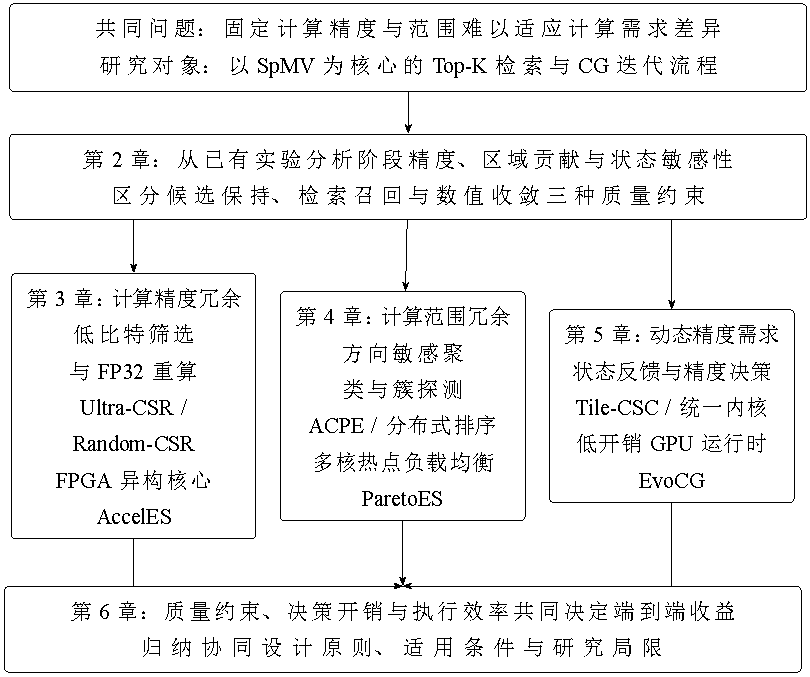
\includegraphics{roadmap.pdf}
\caption{全文研究内容与组织关系}\label{fig:roadmap}
\end{figure}

\subsection{面向计算精度冗余的低比特分层计算方法}
针对大量候选不需要高精度得分却仍参与全量浮点计算的问题，提出 AccelES\cite{jqzhai2025AccelES}。以 INT6 全量粗筛形成候选集合，结合 ReSparse 删除对排序贡献较小的非零元素，再使用 FP32 原始数据进行候选重算。该方法将高精度计算集中到少量相关行，同时保留对候选得分精度的控制。

在执行层，设计适配连续扫描的 Ultra-CSR 和适配候选随机按行访问的 Random-CSR，构建多 Q-core 与 F-core 协同的 FPGA 架构。通过联合设计分层精度机制、阶段化数据表示和异构数据流，将低比特筛选减少的工作量转化为实际访存与执行收益。

\subsection{面向计算范围冗余的结构感知选择性计算方法}
针对 AccelES 的低比特阶段仍需扫描整个候选矩阵的问题，提出 ParetoES\cite{paretoes2026}。采用 Spherical K-means++ Refine 建立与稀疏向量方向相适配的聚类结构，以查询相关簇为单位决定实际访问范围。运行时探测预算使召回率与吞吐率之间的权衡可以在不重新综合硬件的条件下调节。

在执行层，设计自适应簇探测引擎（Adaptive Cluster Probing Engine，ACPE）、分布式微型排序单元及\hbalance{}负载均衡策略，使减少候选访问的算法收益在多 HBM 通道上有效实现。该方法继承第三章的 INT6、Ultra-CSR 与 ReSparse 基础，进一步解决候选空间选择及其引入的不规则执行问题。

\subsection{面向动态精度需求的状态感知混合精度计算方法}
针对迭代状态变化使固定精度难以兼顾性能与收敛的问题，提出 EvoCG\cite{evocg2027}。将搜索方向的局部数值分布作为精度控制输入，通过强化学习选择 FP64、FP32 或 BF16。决策既影响当前 SpMV 成本，也影响后续迭代轨迹，因此以完成求解的总时间及收敛质量为优化依据。

在执行层，设计 Tile-CSC 和统一的线程束级混合精度 SpMV 内核，并以设备端推理、区间复用、融合计算和 CUDA Graph 控制额外开销。该工作将计算需求驱动的协同设计思路拓展至具有状态反馈与误差传播的迭代过程，在保持 CG 计算语义的基础上实现动态精度控制。

\section{论文组织结构}
全文共六章。第1 章介绍背景、相关工作与主要贡献；第2 章结合已有实验分析近似机会和执行瓶颈；第3 章研究低比特分层计算与 FPGA 异构执行；第4 章在此基础上研究候选范围缩减与多核均衡；第5 章拓展至状态反馈驱动的混合精度 CG 与 GPU 执行；第6 章总结结论、适用边界及未来方向。附录列出研究成果、章节对应、符号与复现说明。
